\documentclass[14pt, a4paper]{extarticle}

\usepackage[margin=1in]{geometry}
\usepackage{graphicx}
\usepackage{enumitem}
\usepackage{multicol}
\usepackage{fancyhdr}
\usepackage{amsfonts}
\usepackage{amssymb}
\usepackage{listings}
\usepackage{float}
\usepackage{wrapfig}

\usepackage{gvv-book}
\usepackage{gvv}


\graphicspath{ {figs/} }

\title{MatGeo Assignment 1: 1.5.12}
\author{E Achyuta Siddartha - ee25btech11024}

\begin{document}
\maketitle

\section*{Problem Statement}
In what ratio does the point $\vec{P}(-4, y)$ divide the line segment joining the points $\vec{A}(-6, 10)$ and $\vec{B}(3, -8)$? Hence, find the value of $y$.

\hr

\section*{Solution:}

\subsection*{1. Finding the Ratio}
First, we determine the ratio $m:n$ using the section formula for the known x-coordinate. Let the points be represented by vectors $\vec{a}$, $\vec{b}$, and $\vec{p}$.

Given the x-coordinates $p_x = -4$, $a_x = -6$, and $b_x = 3$:
\begin{align*}
    \vec{p} &= \frac{n\vec{a} + m\vec{b}}{m+n} \\
            &= \frac{7 \myvec{-6 \\ 10} + 2 \myvec{3 \\ -8}}{2+7} \\
            &= \frac{1}{9} \left( \myvec{-42 \\ 70} + \myvec{6 \\ -16} \right) \\
            &= \frac{1}{9} \myvec{-36 \\ 54} \\
            &= \myvec{-4 \\ 6}
\end{align*}
The ratio is $m:n = 2:7$.

\subsection*{2. Finding the Point Coordinates}
Now, using the section formula in vector form with the ratio $2:7$, the desired point $\vec{p}$ is calculated as:
\begin{align*}
    \vec{p} &= \frac{n\vec{a} + m\vec{b}}{m+n} \\
            &= \frac{7 \myvec{-6 \\ 10} + 2 \myvec{3 \\ -8}}{2+7} \\
            &= \frac{1}{9} \left( \myvec{-42 \\ 70} + \myvec{6 \\ -16} \right) \\
            &= \frac{1}{9} \myvec{-36 \\ 54} \\
            &= \myvec{-4 \\ 6}
\end{align*}
The calculation confirms that the x-coordinate is $-4$ and the y-coordinate is $6$.

See the graphical representation in Figure~\ref{fig:line_division}.

\vspace{1cm} % Adds some vertical space

\noindent Therefore, the point $P$ divides the line segment $AB$ in the ratio \textbf{2:7} and the value of $y$ is \textbf{6}.

\begin{figure}[h!]
    \centering
    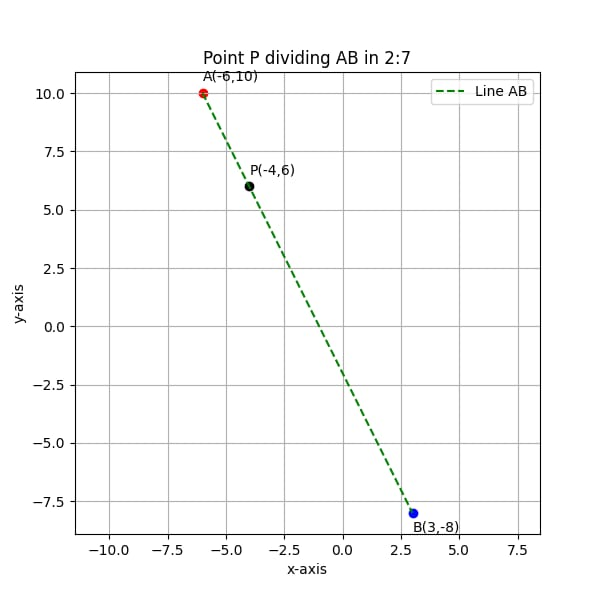
\includegraphics[width=0.7\textwidth]{figs/fig.jpg}
    \caption{Visualization of point $P(-4, 6)$ dividing the line segment joining $A(-6, 10)$ and $B(3, -8)$.}
    \label{fig:line_division}
\end{figure}

\end{document}